\chapter{Analysis}

\section{Artificial Intelligence} % Alternative: AI Models and Prompt Engineering
One of the simplest definitions of an intelligent system is that of a system
that ‘processes information in order to do something purposeful’.\cite{Dignum_2019}






- AI

- machine learning

- deep learning (neural networks)

\subsection{AI Models}
Describe:

Text-to-image, text-to-text, text-to-audio

LLMs - Large Language Models (use neural networks)

GPTs - Generative Pre-Trained Transformers

\subsection{Prompt engineering}
Describe what is

\section{Risks of implementing AI solutions}

\subsection{Ethical risks}
Content generation based on copyrighted material (Copyrighted material as input)

people compromising 

compromising and harmful media 

deep fakes

cyberbullying, fake news

etc.

\subsection{Moral risks}
Sexual / Violent content (inappropriate images, bombs, weapons), forbidden language (illegal activities)

Military use (maybe ethical risk)

etc.

\subsection{Security risks}
social engineering

Malware generation and recursive training of malware samples

Targeted phishing - voice clone, video/image generation of targeted person

etc.

\section{Content filters}
Why are they, and what purpose do they serve

\subsection{Jailbreak}
The specific formulation of the prompt to bypass filters and "jailbreak" the chatbot

jailbreak patching = cat and mouse game

one side develops new jailbreak
    
other patches it and the cycle repeats itself
    



\section{Methods of attacks}
Using the risks to attack

voice cloning, deep fakes, phishing, malware improvement/creation 

\section{Legislation}

\subsection{EU AI Act}
% summary src: https://artificialintelligenceact.eu/high-level-summary/#weglot_switcher



Classification by risk:
Unacceptable risk is prohibited (social scoring systems and manipulative AI)

High-risk AI systems are regulated

limited risk AI systems are subject to lighter transparency obligations: developers and deployers must ensure that end-users are aware that they are interacting with AI (chatbots and deepfakes).

Minimal risk is unregulated

----
General purpose AI (GPAI):

All GPAI model providers must provide technical documentation, instructions for use, comply with the Copyright Directive, and publish a summary of the content used for training.

Free and open licence GPAI model providers only need to comply with copyright and publish the training data summary, unless they present a systemic risk.

All providers of GPAI models that present a systemic risk – open or closed – must also conduct model evaluations, adversarial testing, track and report serious incidents and ensure cybersecurity protections.

- compare / mention others views (i.e. USA, China, basically major countries)
- India, Brasil




% TAKTO SA ROBI FIGURE/OBRAZOK

% Figure \ref{fig:dynabook}:

% \begin{figure}[h]
% \begin{centering}
% 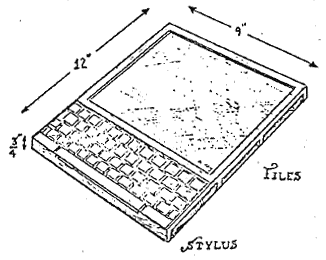
\includegraphics[width=5cm]{assets/images/Dynabook}
% \par\end{centering}
% \caption{Dynabook \label{fig:dynabook}}
% \end{figure}